\documentclass{article}
\usepackage[utf8]{inputenc}
\usepackage[spanish]{babel}
\usepackage{amsmath}
\usepackage{amssymb}
\usepackage{amsfonts}
\usepackage{hyperref}
\usepackage{textcomp}
\usepackage{graphicx}
\usepackage{pgfplots}
\usepackage{geometry}
\usepackage{booktabs}
\hypersetup{
    colorlinks=true,
    linkcolor=black,
    citecolor=green,
    filecolor=magenta,      
    urlcolor=cyan,
}
\geometry{
  top=3cm,
  bottom=3cm,
  left=3cm,
  right=3cm
}

\title{Estadística 1}
\author{Jorge Miguel Alvarado Reyes}
\date{16 Agosto 2023}

\setlength{\parindent}{0pt}
\begin{document}

\begin{titlepage}
    \begin{center}
        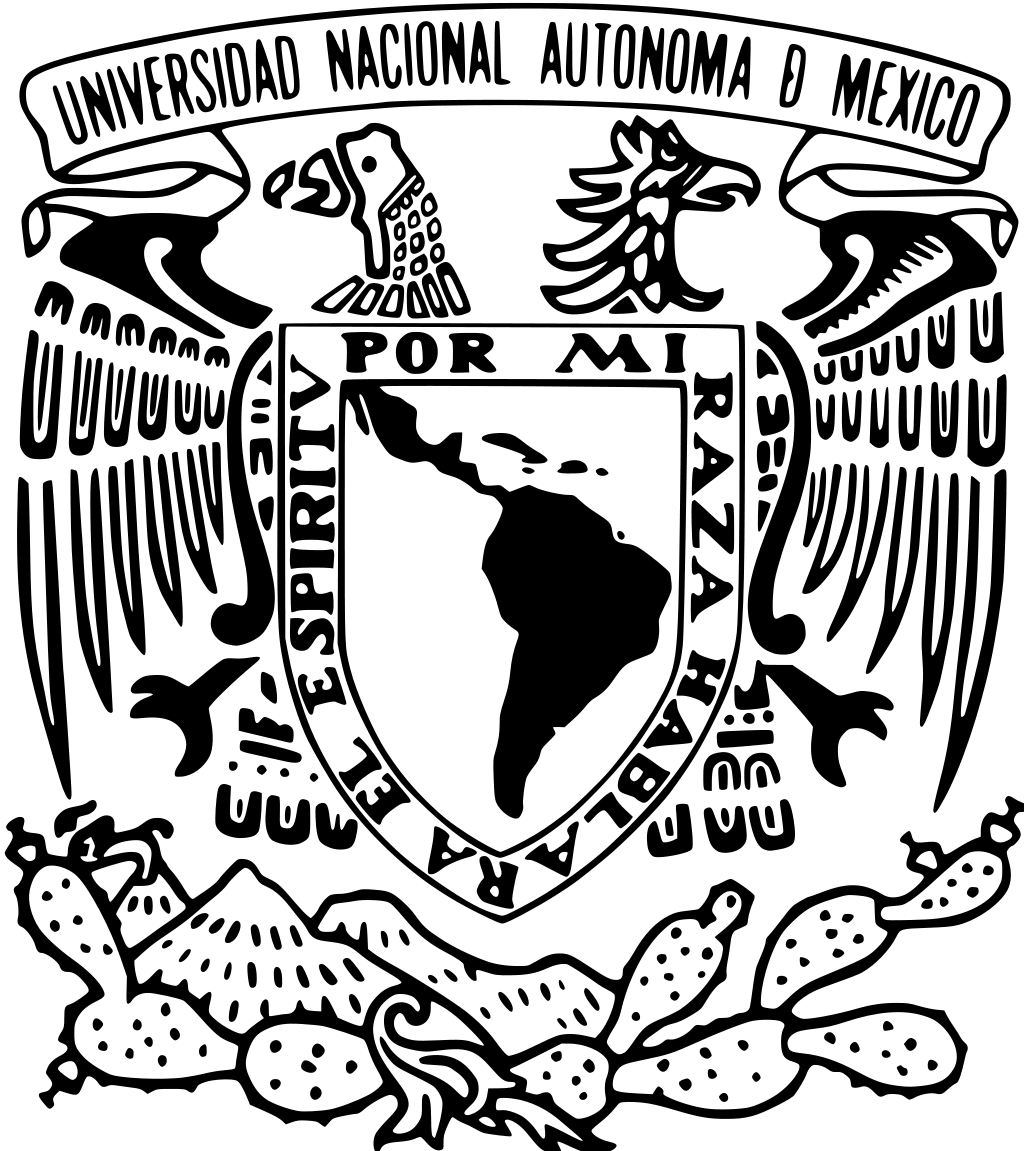
\includegraphics[width=0.2\textwidth]{../../unam.png}
        \vspace*{.5cm}

        \LARGE
        \textbf{Universidad Nacional Autónoma de México}

        \vspace{0.5cm}
        \LARGE
        Facultad de Estudios Superiores Acatlán

        \vspace{2cm}

        \textbf{Apuntes} \\
        Investigación sobre pruebas de normalidad

        \vfill

        \vspace{1cm}

        \textbf{\large Autor:} \\
        Jorge Miguel Alvarado Reyes \\
        \vspace{.5cm}
        \normalsize \today

    \end{center}
\end{titlepage}
\newpage

\tableofcontents

\newpage

\section{Introducción}

La pruebas de normalidad sirven para determinar si los datos de una muestra siguen una distribución normal, Esta distribución es fundamental en estadística debido a que muchos análisis estadísticos asumen que los datos se distribuyen normalmente. Si los datos no cumplen con esta suposición, los resultados de dichos análisis podrían ser engañosos.

\section{Prueba de Lilliefors}

La Prueba de Lilliefors es una modificación de la prueba de Kolmogorov-Smirnov, diseñada específicamente para evaluar la normalidad de una muestra cuando los parámetros de la distribución normal (media y varianza) no son conocidos de antemano. A diferencia de la prueba de Kolmogorov-Smirnov, que requiere que la media y la varianza de la población sean conocidas, la Prueba de Lilliefors estima estos parámetros directamente de los datos de la muestra.

La hipótesis nula se rechaza si la estadística de prueba calculada excede un valor crítico, lo cual indica una discrepancia significativa entre la distribución de la muestra y una distribución normal teórica. La estadística de prueba se basa en la máxima diferencia absoluta entre la función de distribución empírica de la muestra y la función de distribución acumulativa normal ajustada, como se muestra en la fórmula siguiente:

\[
    D = \max | F_n(x) - F(x; \hat{\mu}, \hat{\sigma}) |
\]

donde:
\begin{itemize}
    \item \(D\) es la máxima diferencia absoluta entre la función de distribución empírica \(F_n(x)\) y la función de distribución acumulativa normal \(F(x; \hat{\mu}, \hat{\sigma})\).
    \item \(F_n(x)\) representa la función de distribución empírica basada en los datos de la muestra.
    \item \(F(x; \hat{\mu}, \hat{\sigma})\) es la función de distribución acumulativa normal teórica, con la media \(\hat{\mu}\) y la varianza \(\hat{\sigma}\) estimadas a partir de los datos de la muestra.
\end{itemize}

Para llevar a cabo la Prueba de Lilliefors en el entorno de R, se puede utilizar el comando \texttt{lillie.test} del paquete \texttt{nortest}.


\section{Prueba de Cramér-van Mises}

La Prueba de Cramér-van Mises es un método estadístico utilizado para evaluar la hipótesis de que una muestra dada se distribuye de acuerdo con una distribución teórica específica. A diferencia de otras pruebas de bondad de ajuste, esta prueba considera la diferencia cuadrada entre la función de distribución acumulada empírica de la muestra y la teórica, integrada a lo largo de todo el rango de los datos. Es especialmente útil para análisis en los que se requiere una estimación de distancia mínima y puede aplicarse en dos contextos principales: una muestra y dos muestras.

\subsection*{Una Muestra}

Para una muestra, la estadística de prueba se calcula mediante la fórmula:

\[
    T = nw^2 = \frac{1}{12n} + \sum_{i=1}^{n}\left[\frac{2i - 1}{2n} - F(x_i)\right]^2
\]

donde \(F\) es la función de distribución acumulada teórica y \(x_i\) son los valores observados, ordenados de manera creciente. Si el valor calculado de \(T\) excede el valor crítico tabulado, se rechaza la hipótesis nula de que los datos siguen la distribución \(F\).

\subsection*{Dos Muestras}

En el contexto de dos muestras, la prueba compara las distribuciones empíricas de dos conjuntos de datos para evaluar si provienen de la misma distribución subyacente. La estadística de prueba para dos muestras se calcula como:

\[
    U^2 = \frac{n m}{n + m} \int_{-\infty}^{\infty} [F_n(x) - G_m(x)]^2 dH(x)
\]

donde:
\begin{itemize}
    \item \(n\) y \(m\) son los tamaños de las dos muestras.
    \item \(F_n(x)\) es la función de distribución acumulada empírica de la primera muestra.
    \item \(G_m(x)\) es la función de distribución acumulada empírica de la segunda muestra.
    \item \(H(x)\) es la función de distribución acumulada empírica combinada de ambas muestras.
    \item La integración se realiza a lo largo de todo el rango de los datos.
\end{itemize}

Un valor grande de \(U^2\) indica una evidencia significativa contra la hipótesis nula de que las dos muestras provienen de la misma distribución subyacente.


\section{Prueba de Shapiro-Wilk}

Sirve para determinar si un conjunto de datos se distribuye normalmente, fue publicada en 1965 por Samuel Shapiro y Martin Wilk, esta prueba es considerada como una de las más potentes para el contraste de normalidad.

La hipótesis nula ($H_0$) plantea que la muestra proviene de una población normalmente distribuida. El estadístico de prueba W se calcula a partir de los datos de la muestra, utilizando una fórmula específica que involucra los valores ordenados de la muestra, la media muestral y ciertas constantes $a_i$, que se derivan de las covarianzas, varianzas y medias de una muestra normalmente distribuida. La prueba tiene un rango para $W$ de 0 a 1, y la hipótesis nula se rechaza si W es demasiado pequeño, indicando que la distribución de los datos no es normal

\[W = \frac{\left(\sum_{i=1}^{n}a_{i}x_{(i)}\right)^{2}}{\sum_{i=1}^{n}(x_{i}-\overline{x})^{2}}
\]

Aunque la prueba de Shapiro-Wilk es altamente eficaz, tiene limitaciones, especialmente en muestras muy grandes, donde puede ser demasiado sensible a desviaciones insignificantes de la normalidad. Por esta razón, es importante considerar el contexto y el tamaño de la muestra al interpretar los resultados.

En R se puede realizar la prueba con la función shapiro.test.

\section{Prueba de Anderson-Darling}

La prueba de Anderson-Darling es un método estadístico utilizado para evaluar si un conjunto de datos sigue una distribución específica. Aunque se aplica comúnmente para verificar la normalidad de los datos, la prueba puede utilizarse para otras distribuciones como la exponencial, la Weibull, entre otras.

El núcleo de esta prueba radica en dos hipótesis fundamentales:

\begin{itemize}
    \item Hipótesis nula (\(H_0\)): Los datos se ajustan a la distribución específica.
    \item Hipótesis alternativa (\(H_1\)): Los datos no se ajustan a la distribución específica.
\end{itemize}

El estadístico de prueba se calcula de la siguiente manera, donde la fórmula ajusta el enfoque según la distribución de interés.
\[A^2 = -n - \frac{1}{n} \sum_{i=1}^{n} (2i-1) \left[ \ln(F(x_i)) + \ln(1-F(x_{n+1-i})) \right]\]

Donde \(n\) es el tamaño de la muestra, \(x_i\) son los datos ordenados y \(F\) es la función de distribución acumulada teórica.

La interpretación de los resultados de la prueba de Anderson-Darling se basa en el valor \(p\) obtenido: un valor \(p\) bajo (por lo general, menor que 0.05) sugiere el rechazo de la hipótesis nula, indicando que los datos no se ajustan a la distribución especificada.

\section{Prueba de Jarque-Bera}

La prueba de Jarque-Bera es una herramienta estadística de bondad de ajuste que evalúa si una muestra de datos tiene las características de asimetría y curtosis que se esperarían de una distribución normal. Desarrollada por Carlos Jarque y Anil K. Bera, esta prueba es especialmente valiosa para analizar grandes muestras de datos. A diferencia de otras pruebas de normalidad, como la prueba de Shapiro-Wilk, que pueden perder precisión con tamaños de muestra muy grandes (por ejemplo, más de 2000 observaciones), la prueba de Jarque-Bera mantiene su fiabilidad incluso en estos casos.

La prueba de Jarque-Bera se basa en la comparación de la asimetría y curtosis de los datos de la muestra con los valores esperados en una distribución normal (asimetría de cero y curtosis de tres), lo cual indica una distribución perfectamente simétrica alrededor de la media. La estadística de prueba de Jarque-Bera se calcula como sigue:

\[JB = \frac{n}{6} \left(S^2 + \frac{1}{4}(K - 3)^2\right)\]

donde \(n\) es el número de observaciones, \(S\) es la asimetría de la muestra, y \(K\) es la curtosis de la muestra. Bajo la hipótesis nula (H0), se asume que los datos siguen una distribución normal. La hipótesis alternativa (H1) es que los datos no siguen una distribución normal. Un valor alto en la estadística JB indica una desviación significativa de la normalidad, sugiriendo el rechazo de la hipótesis nula.

Para llevar a cabo la prueba de Jarque-Bera en R, se pueden utilizar paquetes como \texttt{tseries} con la función \texttt{jarque.bera.test}, o el paquete \texttt{moments} con la función \texttt{jarque.test}. Estas herramientas facilitan la aplicación de la prueba en análisis estadísticos, permitiendo a los investigadores evaluar la adecuación de la normalidad en sus conjuntos de datos, especialmente útil en campos como la econometría y la investigación financiera, donde la normalidad de los retornos es una suposición común.

\section{Conclusiones}

Este documento ha explorado diversas pruebas de normalidad, destacando su importancia en el análisis estadístico. La normalidad de los datos es una suposición clave en muchos métodos estadísticos, incluyendo pruebas paramétricas y modelos de regresión. Las pruebas de Shapiro-Wilk, Lilliefors, Cramér-van Mises, Anderson-Darling, y Jarque-Bera ofrecen diferentes enfoques para evaluar esta suposición, cada una con sus propias ventajas y limitaciones.

Una lección clave es la necesidad de seleccionar la prueba de normalidad más adecuada basada en el tamaño de la muestra y las características específicas de los datos. Por ejemplo, la prueba de Shapiro-Wilk es preferida para muestras pequeñas, mientras que la prueba de Jarque-Bera es más adecuada para muestras grandes. La Prueba de Lilliefors y la Prueba de Anderson-Darling son útiles cuando los parámetros de la distribución normal no son conocidos, y la Prueba de Cramér-van Mises ofrece una alternativa robusta que evalúa la bondad de ajuste para cualquier distribución teórica.

El correcto uso de estas pruebas permite a los investigadores y analistas tomar decisiones informadas sobre la aplicabilidad de métodos estadísticos que asumen normalidad. Cuando los datos no se ajustan a una distribución normal, pueden considerarse transformaciones de los datos o métodos no paramétricos como alternativas válidas.

Finalmente, este documento subraya la importancia de la comprensión profunda de las pruebas de normalidad dentro del contexto de investigación específico. Una interpretación adecuada de sus resultados es crucial para la validez de las conclusiones estadísticas y, en última instancia, para el avance del conocimiento en diversas áreas de aplicación.

En resumen, las pruebas de normalidad son herramientas esenciales en el arsenal estadístico, facilitando la correcta aplicación y interpretación de técnicas analíticas avanzadas. Su elección y aplicación cuidadosa asegura la fiabilidad y validez de los resultados estadísticos en investigación.


\end{document}